\chapter{Einleitung}

\section{Motivation}

Die Motivation der Arbeit war das Vertiefen der vermittelten, theoretischen Inhalte. Erwartet wurde kein umfangreiches Projekt, sondern nur ein kleines, auf einem 8051 Mikrocomputer lauffähiges Programm, welches ein wenig über den vermittelten Lernstoff hinaus reicht und damit das Wissen um Assembler\cite{bib:assembler} weiter festigt und vertieft.

\section{Aufgabenstellung}

Die Aufgabe war es mit dem erworbenen Wissen aus der Vorlesung \zitat{Systemnahe Programmierung} ein kleines Programm zu entwickeln. Dieses soll dann auf einem 8051 Mikrocomputer mit simulierter Hardware laufen. Die Simulation selbst wird von der verwendeten Entwicklungsumgebung MCU-8051 IDE bereitgestellt. Der 8051 und die IDE werden in Kapitel \ref{section:8051} und \ref{section:ide} genauer vorgestellt.

Wir als Gruppe haben uns das Ziel gesetzt, das bekannte \zitat{Bombenspiel} zu entwickeln. Hierbei wird eine Bombe mit zufälliger Zündschnur zwischen zwei Spielern hin und her geworfen. Der Spieler, bei dem die Bombe explodiert, hat verloren. Das genaue Konzept zu unserer Idee ist in Kapitel \ref{section:konzept} ausführlich erklärt.

\section{Der 8051 Mikrocomputer} \label{section:8051}

Der 8051 Mikrocomputer wurde 1981 von Intel als 8-bit Mikrocontroller auf den Markt gebracht. Es handelt sich um ein \zitat{system on a chip}, was bedeutet, dass RAM, ROM, zwei Timer, ein Serial Port, 4 8-bit Ports und noch einiges mehr auf einem einzigen Chip verbaut sind. Die einzelnen Bestandteile sind in Abbildung \ref{img:8051} dargestellt.\cite{bib:8051}

Mittlerweile ist der Original 8051 veraltet, dennoch existieren viele Abwandlungen (Derivate) beziehungsweise Weiterentwicklungen des 8051. Diese sind allerdings mit höherer Taktfrequenz und geringerer Taktteilung ausgestattet, sodass sie nahezu auf dem aktuellen Stand der Technik und damit deutlich leistungsfähiger als das Ursprungsmodell sind.\cite{bib:8051_2}

\begin{figure}[htbp]
	\centering
	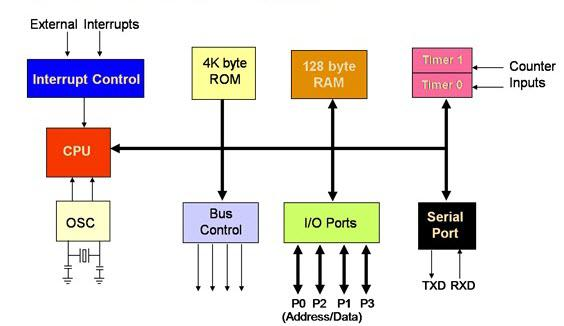
\includegraphics[scale=0.75]{img/8051-diagram}
	\caption{Blockdiagramm eines 8051 Mikrocomputers}
	\label{img:8051}
	\source{https://www.tutorialspoint.com/embedded_systems/images/block_diagram.jpg}
\end{figure}
